\documentclass[14pt, a4paper]{extarticle}
\usepackage[T2A]{fontenc}
\usepackage[utf8]{inputenc}
\usepackage[english,russian]{babel}
\usepackage[left = 3cm, right = 1cm, top = 2cm, bottom = 2cm]{geometry}
\setlength\parindent{12.5mm} 
\linespread{1.3}
\usepackage{enumitem}
\usepackage{amsmath}
\usepackage{amssymb}
\usepackage{wrapfig}
\usepackage{indentfirst}
\usepackage{hyperref} % ДОЛЖЕН БЫТЬ ПОСЛЕДНИМ (кроме cleveref)
\hypersetup{
	colorlinks=true,
	citecolor=blue,
	urlcolor=blue, 
	linkcolor=blue,
	pdfencoding=auto
}
\usepackage{xcolor}   % Пакет для работы с цветами
\usepackage{listings} % Пакет для оформления кода
\usepackage{graphicx}
\usepackage{float}
\usepackage{longtable}
\usepackage[htt]{hyphenat}
% Определяем приглушенные цвета для академического стиля
\definecolor{codegreen}{rgb}{0,0.6,0}
\definecolor{codegray}{rgb}{0.5,0.5,0.5}
\definecolor{codepurple}{rgb}{0.58,0,0.82}
\definecolor{backcolour}{rgb}{0.97,0.97,0.97}
% Глобальная настройка стиля листингов
\lstset{ 
	language=C++,                       % Указываем язык по умолчанию
	backgroundcolor=\color{backcolour}, % Светло-серый фон
	commentstyle=\color{codegreen}\itshape, % Комментарии зеленым курсивом
	keywordstyle=\color{blue}\bfseries, % Ключевые слова синим и жирным
	numberstyle=\tiny\color{codegray},  % Стиль номеров строк (мелкий, серый)
	stringstyle=\color{codepurple},     % Строки фиолетовым
	basicstyle=\ttfamily\footnotesize,  % Моноширинный шрифт, чуть меньше основного
	breakatwhitespace=false,         
	breaklines=true,                    % Автоматический перенос длинных строк
	captionpos=t,                       % Позиция заголовка (t - сверху, b - снизу)
	keepspaces=true,                 
	numbers=left,                       % Номера строк слева
	numbersep=10pt,                     % Отступ номеров от кода
	showspaces=false,                
	showstringspaces=false,
	showtabs=false,                  
	tabsize=4,                          % Размер табуляции
	frame=single,                       % Одинарная рамка вокруг кода
	rulecolor=\color{black!30},          % Цвет рамки (светло-серый)
	extendedchars=\true
}
\newcommand{\tab}{\hspace{12.5mm}}

\usepackage{tabularx} % Обязательный пакет для этого способа

% Создаем команду для удобного центрирования текста внутри растягиваемых ячеек
\newcolumntype{Y}{>{\centering\arraybackslash}X}

\begin{document}
\thispagestyle{empty}
\begin{center}
    \hspace{0.2cm}МИНИСТЕРСТВО НАУКИ И ВЫСШЕГО ОБРАЗОВАНИЯ РОССИЙСКОЙ ФЕДЕРАЦИИ\\
    Федеральное государственное автономное образовательное\\
    учреждение высшего образования\\
    {\bf <<Санкт-Петербургский политехнический\\
    университет Петра Великого>>}\\
    Институт компьютерных наук и кибербезопасности\\
    Высшая школа технологий искусственного интеллекта\\
    02.03.01\_03 Технологии машинного обучения и искусственного интеллекта\\
    \vspace{3cm}
    \Large\bf{
        Отчёт о выполнении лабораторной работы №3\\
        Основы архитектуры ЦВМ\\[1cm]
    }
\end{center}
\vspace{2cm}
\begin{flushleft}
    {\bf Выполнил:}\\
    Cтудент группы 5130201/50302 \hfill
    \line(1,0){4cm} \quad Калинский В.И.\\
    {\bf Принял:}\\
    К.т.н., доцент, доцент ВШТИИ и КОЦ ИИ \hfill
    \line(1,0){3 cm} \quad Вербова Н.М.\\[0.5cm]
    { \hfill<<\rule{1cm}{0.5pt}>>\rule{2cm}{0.5pt}\hspace{3pt}2026 г.}
\end{flushleft}
\vspace{1cm}
\begin{center}
    Санкт-Петербург, 2026
\end{center}
\newpage
\textbf{
	\\Цель работы:}

\noindent Изучить принципы синтеза последовательных схем на примере синтеза недвоичного счётчика.
\\\\
\textbf{Методика: }

Необходимо было синтезировать недвоичный вычитающий счётчик с коэффициентом пересчёта $K_\text{сч} = 5$. Число триггеров $m$ рассчитывается по формуле объёма памяти:
$m \ge |\log_2 K_\text{сч}| = |\log_2 5| = 2.32 => m = 3\text{ триггера}$. Число избыточных состояний: $N = 2^m - K_{\text{сч}} = 2^3 - 5 = 3$. После исключения 3 состояний счётчика была составлена таблица функционирования счётчика (таблица \ref{tab:1}).

\begin{table}[h!]
	\centering
	% Указываем 11 столбцов типа Y для автоматического распределения по всей ширине
	\begin{tabular}{|c|c|c|c|c|c|c|}
		\hline
		№ сост. & $Q_1^t$ & $Q_2^t$ & $Q_3^t$ & $Q_1^{t+1}$ & $Q_2^{t+1}$ & $Q_3^{t+1}$ \\ \hline
		4 &	1 & 0 & 0 & 0 & 1 & 1 \\ \hline
		3 &	0 & 1 & 1 & 0 & 1 & 0 \\ \hline
		2 &	0 & 1 & 0 & 0 & 0 & 1 \\ \hline
		1 &	0 & 0 & 1 & 0 & 0 & 0 \\ \hline
		0 &	0 & 0 & 0 & 1 & 0 & 0 \\ \hline
	\end{tabular}
	\caption{Таблица переходов триггеров}
	\label{tab:1}
\end{table}

На основе таблицы \ref{tab:1} были построены прикладные таблицы счётчика.
\begin{center}
	\small
	\setlength{\tabcolsep}{4.5pt}
	\begin{minipage}{0.32\textwidth}
		\centering
		\textbf{$Q_1^t \to Q_1^{t+1}$}\\[4pt]
		\begin{tabular}{|c|c|c|c|c|}
			\hline
			& \multicolumn{2}{c|}{$Q_2$} & \multicolumn{2}{c|}{$\overline{Q}_2$} \\ \hline
			$Q_3$ & 00 & -- & -- & 00 \\ \hline
			$\overline{Q}_3$ & 00 & -- & 10 & 01 \\ \hline
			& $\overline{Q}_1$ & $Q_1$ & $Q_1$ & $\overline{Q}_1$ \\ \hline
		\end{tabular}
	\end{minipage}
	\hfill
	\begin{minipage}{0.32\textwidth}
		\centering
		\textbf{$Q_2^t \to Q_2^{t+1}$}\\[4pt]
		\begin{tabular}{|c|c|c|c|c|}
			\hline
			& \multicolumn{2}{c|}{$Q_2$} & \multicolumn{2}{c|}{$\overline{Q}_2$} \\ \hline
			$Q_3$ & 11 & -- & -- & 00 \\ \hline
			$\overline{Q}_3$ & 10 & -- & 01 & 00 \\ \hline
			& $\overline{Q}_1$ & $Q_1$ & $Q_1$ & $\overline{Q}_1$ \\ \hline
		\end{tabular}
	\end{minipage}
	\hfill
	\begin{minipage}{0.32\textwidth}
		\centering
		\textbf{$Q_3^t \to Q_3^{t+1}$}\\[4pt]
		\begin{tabular}{|c|c|c|c|c|}
			\hline
			& \multicolumn{2}{c|}{$Q_2$} & \multicolumn{2}{c|}{$\overline{Q}_2$} \\ \hline
			$Q_3$ & 10 & -- & -- & 10 \\ \hline
			$\overline{Q}_3$ & 01 & -- & 01 & 00 \\ \hline
			& $\overline{Q}_1$ & $Q_1$ & $Q_1$ & $\overline{Q}_1$ \\ \hline
		\end{tabular}
	\end{minipage}
\end{center}

Далее были составлены карты Карно согласно характеристической таблице для J-K триггера (таблица \ref{tab:jk}). По ним были составлены аналитические выражения.
\begin{center}
	\begin{tabular}{|c|c|c|}
		\hline
		$Q^t \rightarrow Q^{t+1}$ & $J^t$ & $K^t$ \\ \hline
		00 & 0 & * \\ \hline
		01 & 1 & * \\ \hline
		10 & * & 1 \\ \hline
		11 & * & 0 \\ \hline
	\end{tabular}
	\label{tab:jk}
\end{center}

\noindent Далее были составлены карты Карно для $J$-входов и $K$-входов. Жирным отмечены контуры.
\begin{center}
	\small	
	\begin{minipage}{0.32\textwidth}
		\centering
		\textbf{$J_1$}\\[4pt]
		\begin{tabular}{|c|c|c|c|c|}
			\hline
			& \multicolumn{2}{c|}{$Q_2$} & \multicolumn{2}{c|}{$\overline{Q}_2$} \\ \hline
			$Q_3$ & 0 & * & * & 0 \\ \hline
			$\overline{Q}_3$ & 0 & * & \textbf{*} & \textbf{1} \\ \hline
			& $\overline{Q}_1$ & $Q_1$ & $Q_1$ & $\overline{Q}_1$ \\ \hline
		\end{tabular}
	\end{minipage}
	\hfill
	\begin{minipage}{0.32\textwidth}
		\centering
		\textbf{$J_2$}\\[4pt]
		\begin{tabular}{|c|c|c|c|c|}
			\hline
			& \multicolumn{2}{c|}{$Q_2$} & \multicolumn{2}{c|}{$\overline{Q}_2$} \\ \hline
			$Q_3$ & * & \textbf{*} & \textbf{*} & 0 \\ \hline
			$\overline{Q}_3$ & * & \textbf{*} & \textbf{1} & 0 \\ \hline
			& $\overline{Q}_1$ & $Q_1$ & $Q_1$ & $\overline{Q}_1$ \\ \hline
		\end{tabular}
	\end{minipage}
	\hfill
	\begin{minipage}{0.32\textwidth}
		\centering
		\textbf{$J_3$}\\[4pt]
		\begin{tabular}{|c|c|c|c|c|}
			\hline
			& \multicolumn{2}{c|}{$Q_2$} & \multicolumn{2}{c|}{$\overline{Q}_2$} \\ \hline
			$Q_3$ & \textbf{*} & \textbf{*} & \textbf{*} & * \\ \hline
			$\overline{Q}_3$ & \textbf{1} & \textbf{*} & \textbf{1} & 0 \\ \hline
			& $\overline{Q}_1$ & $Q_1$ & $Q_1$ & $\overline{Q}_1$ \\ \hline
		\end{tabular}
	\end{minipage}
	\title{карты Карно для $J$-входов}
\end{center}

\vspace{0.3cm}

\begin{center}
	\small	
	\begin{minipage}{0.32\textwidth}
		\centering
		\textbf{$K_1$}\\[4pt]
		\begin{tabular}{|c|c|c|c|c|}
			\hline
			& \multicolumn{2}{c|}{$Q_2$} & \multicolumn{2}{c|}{$\overline{Q}_2$} \\ \hline
			$Q_3$ & \textbf{*} & \textbf{*} & \textbf{*} & \textbf{*} \\ \hline
			$\overline{Q}_3$ & \textbf{*} & \textbf{*} & \textbf{1} & \textbf{*} \\ \hline
			& $\overline{Q}_1$ & $Q_1$ & $Q_1$ & $\overline{Q}_1$ \\ \hline
		\end{tabular}
	\end{minipage}
	\hfill
	\begin{minipage}{0.32\textwidth}
		\centering
		\textbf{$K_2$}\\[4pt]
		\begin{tabular}{|c|c|c|c|c|}
			\hline
			& \multicolumn{2}{c|}{$Q_2$} & \multicolumn{2}{c|}{$\overline{Q}_2$} \\ \hline
			$Q_3$ & 0 & * & * & * \\ \hline
			$\overline{Q}_3$ & \textbf{1} & \textbf{*} & \textbf{*} & \textbf{*} \\ \hline
			& $\overline{Q}_1$ & $Q_1$ & $Q_1$ & $\overline{Q}_1$ \\ \hline
		\end{tabular}
	\end{minipage}
	\hfill
	\begin{minipage}{0.32\textwidth}
		\centering
		\textbf{$K_3$}\\[4pt]
		\begin{tabular}{|c|c|c|c|c|}
			\hline
			& \multicolumn{2}{c|}{$Q_2$} & \multicolumn{2}{c|}{$\overline{Q}_2$} \\ \hline
			$Q_3$ & \textbf{1} & \textbf{*} & \textbf{*} & \textbf{1} \\ \hline
			$\overline{Q}_3$ & \textbf{*} & \textbf{*} & \textbf{*} & \textbf{*} \\ \hline
			& $\overline{Q}_1$ & $Q_1$ & $Q_1$ & $\overline{Q}_1$ \\ \hline
		\end{tabular}
	\end{minipage}
	\title{карты Карно для $K$-входов}
\end{center}

По результатам склеивания контуров в картах Карно получена следующая система уравнений:
\begin{align*}
	J_1 &= \overline{Q}_2 \cdot \overline{Q}_3, & K_1 &= 1, \\
	J_2 &= Q_1, & K_2 &= \overline{Q}_3, \\
	J_3 &= Q_1 + Q_2, & K_3 &= 1.
\end{align*}

Согласно полученным уравнениям была синтезирована схема, приведённая на рис. \ref{fig:3-1}.
\begin{figure}[H]
	\centering
	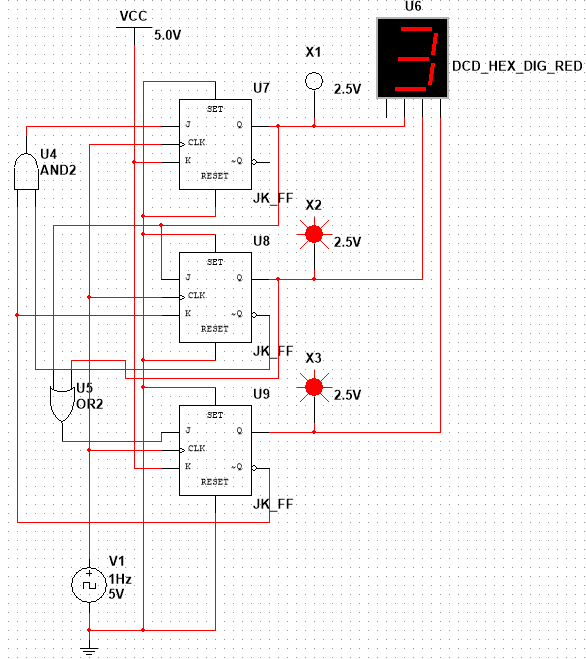
\includegraphics[width=0.7\linewidth]{3-1}
	\caption{Схема недвоичного вычитающего счётчика с коэффициентом пересчёта $K_\text{сч} = 5$}
	\label{fig:3-1}
\end{figure}

Во второй части лабораторной работы необходимо было изучить принцип работы счётчика ИС К155ИЕ6 (SN74192). На основе схемы для исследования ИС К155ИЕ6 (рис. \ref{fig:p11}) была синтезирована схема, приведённая на рис. \ref{fig:3-2}. 

\begin{figure}[H]
	\centering
	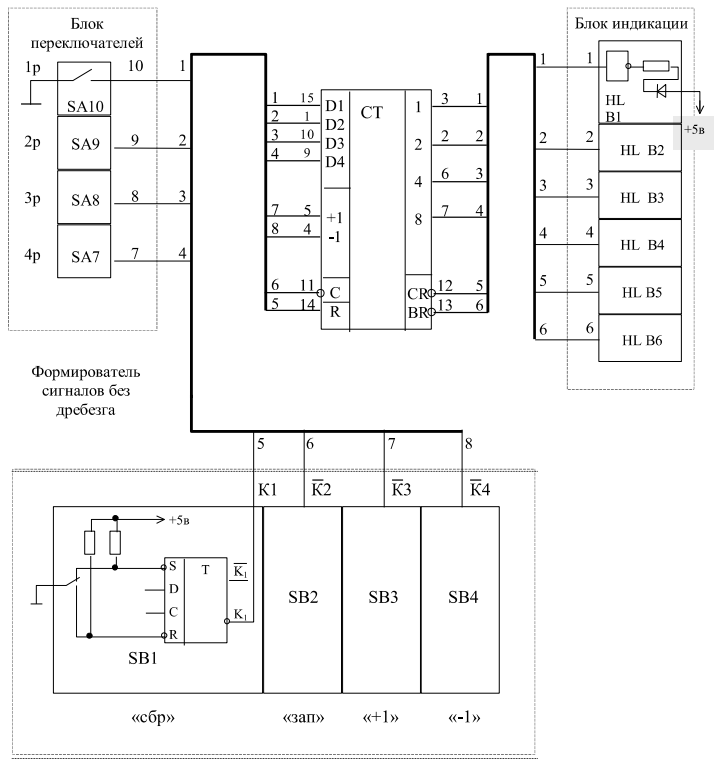
\includegraphics[width=0.7\linewidth]{p11}
	\caption{Схема для исследования ИС К155ИЕ6 (SN74192)}
	\label{fig:p11}
\end{figure}

\begin{figure}[H]
	\centering
	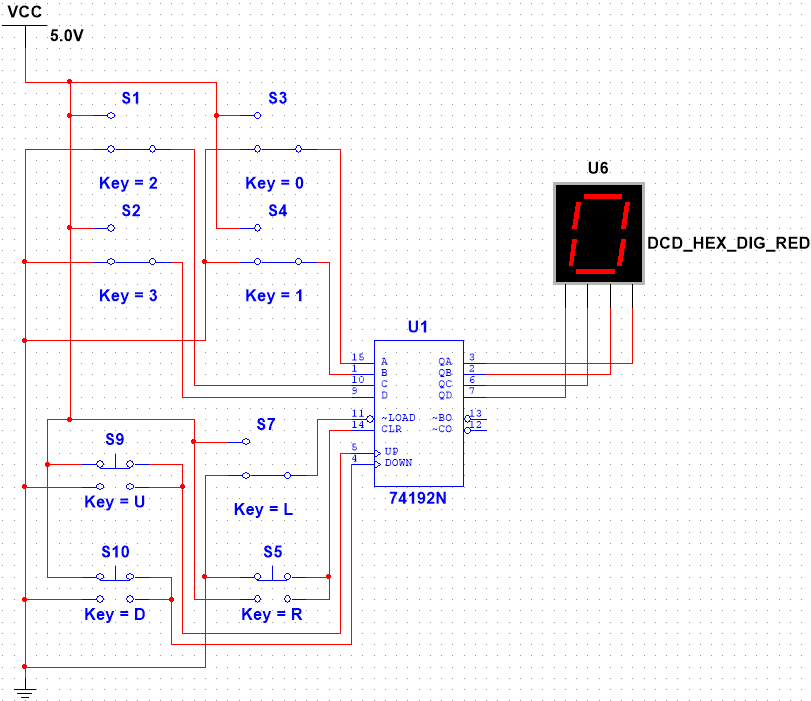
\includegraphics[width=0.7\linewidth]{3-2}
	\caption{Схема счётчика ИС К155ИЕ6 (SN74192)}
	\label{fig:3-2}
\end{figure}

Далее подключён вход «+1» к выходу функционального генератора, чтобы исследовать работу счётчика при суммировании в динамике. Требовалось подключить входы логического анализатора к выходам триггеров первого (1), второго (2), третьего (4) и четвёртого (8) разрядов счётчика. Полученная схема отражена на рис. \ref{fig:oscilscheme}, а осциллограммы сигналов на выходах счётчика -- на рис. \ref{fig:oscillog1}.

\begin{figure}
	\centering
	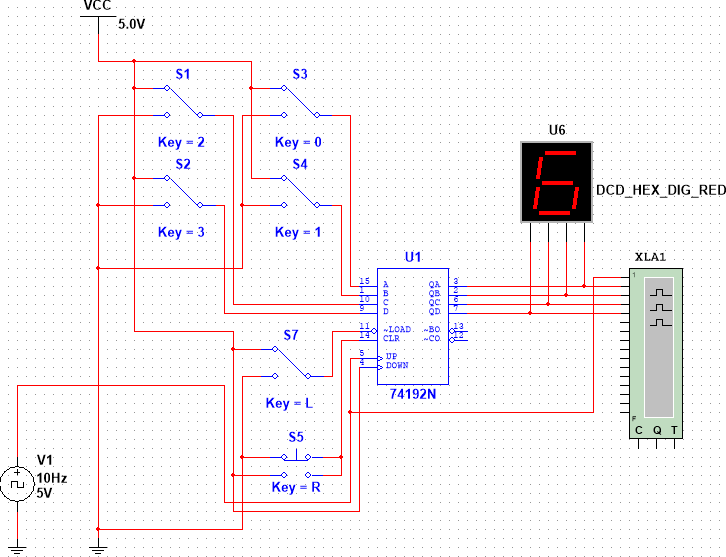
\includegraphics[width=0.7\linewidth]{oscilscheme.png}
	\caption{Изменённая схема счётчика ИС К155ИЕ6 (SN74192)}
	\label{fig:oscilscheme}
\end{figure}

\begin{figure}[H]
	\centering
	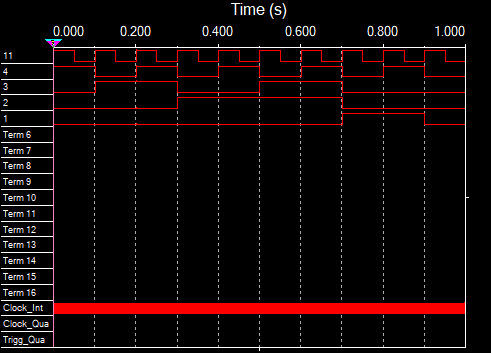
\includegraphics[width=0.7\linewidth]{oscillog1}
	\caption{Осциллограммы сигналов на выходах счётчика}
	\label{fig:oscillog1}
\end{figure}

Следующая часть лабораторной работы -- создание суммирующего счётчика с $K_\text{сч} = 6$ на базе микросхемы К155ИЕ6 (SN74192). По умолчанию микросхема считает до 10 (от 0 до 9), необходимо ограничить её счёт шестью состояниями ($K_\text{сч} = 6$):
$$0 \to 1 \to 2 \to 3 \to 4 \to 5 \to 0 \dots$$
В момент, когда счётчик пытается переключиться на следующее число -- 6, дешифратор должен выдать короткий импульс на вход сброса CLR, сбросив счётчик обратно в 0. Нужно синтезировать дешифратор, который выдаёт 1 при 6 (бинарная 0110): $F = \overline{Q}_D \cdot Q_C \cdot Q_B \cdot \overline{Q}_A$. Полученная схема отражена на рис. \ref{fig:3-3}.

\begin{figure}[H]
	\centering
	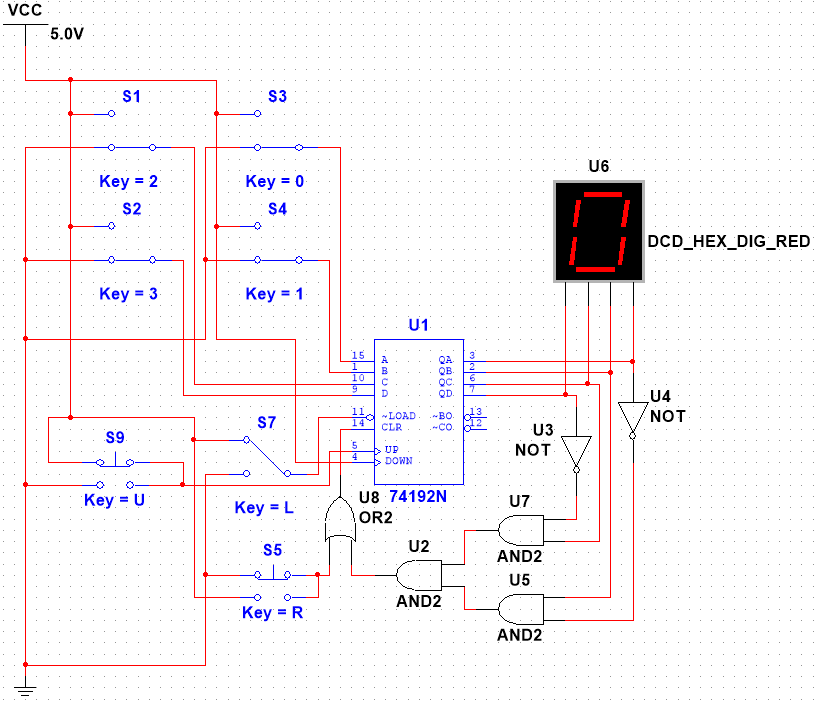
\includegraphics[width=0.7\linewidth]{3-3}
	\caption{Cхема счётчика ИС К155ИЕ6 (SN74192) для $K_\text{сч} = 6$}
	\label{fig:3-3}
\end{figure}

\textbf{Выводы}

В ходе выполнения лабораторной работы были изучены принципы построения и функционирования последовательностных логических устройств: триггеров и счётчиков импульсов различной разрядности. С помощью карт Карно для J-K триггеров был синтезирован синхронный вычитающий счётчик ($K_{сч} = 5$), подтвердивший при моделировании в Multisim соответствие расчётам и свойство самовосстановления. Также было исследовано функционирование интегрального двоично-десятичного счётчика К155ИЕ6 (74192) в режимах сброса, параллельной загрузки и реверсивного счёта со снятием осциллограмм. Синтез дешифратора состояния на логических элементах позволил модифицировать схему под суммирующий счёт с $K_{сч} = 6$, что наглядно продемонстрировало принципы управления коэффициентом пересчёта в цифровых вычислительных устройствах.

%КАРТИНКИ
%\begin{figure}[H]
%	\centering
%	\includegraphics[width=0.85\textwidth]{install_deb.png}
%	\caption{Начало установки гостевой ОС Debian 12}
%	\label{fig:vbox_setup}
%\end{figure}

%---------------------------------------------------------------------------------
%ССЫЛКИ НА САЙТ

%\href{https://www.virtualbox.org/wiki/Downloads}{официального сайта VirtualBox}

%---------------------------------------------------------------------------------
%ССЫЛКА НА ПРИЛОЖЕНИЕ

%\texttt{zlib}\cite{zlib_docs}

%---------------------------------------------------------------------------------
%ССЫЛКА НА РИСУНОК

%показано на рис. \ref{fig:vbox_setup}

%---------------------------------------------------------------------------------
%ТАБЛИЦА С ПЕРЕВОДОМ НА СЛЕДУЮЩУЮ СТРАНИЦУ

%\begin{longtable}{|l|p{0.75\textwidth}|}
%	\caption{Функции библиотеки ncurses, используемые в TUI} \label{tab:ncurses_funcs} \\
%	\hline
%	\textbf{Функция} & \textbf{Назначение и описание алгоритма работы} \\ \hline
%	\endhead
%	\texttt{initscr()} & Инициализирует библиотеку, выделяет память под внутренние структуры окна и переводит терминал ОС в графический режим. \\ \hline
%	\texttt{cbreak()} & Отключает строковую буферизацию терминала, позволяя программе мгновенно реагировать на нажатия клавиш без ожидания \texttt{Enter}. \\ \hline
%	\texttt{noecho()} & Отключает автоматический вывод (эхо) вводимых пользователем символов на экран, позволяя программе самой управлять отрисовкой. \\ \hline
%	\texttt{clear()} & Очищает виртуальный экран для подготовки к отрисовке нового кадра меню. \\ \hline
%	\texttt{move(y, x)} & Осуществляет абсолютное позиционирование курсора по координатам \texttt{Y} (строка) и \texttt{X} (столбец). \\ \hline
%	\texttt{printw()} & Аналог функции \texttt{printf} для \texttt{ncurses}: выводит отформатированный текст в текущей позиции курсора. \\ \hline
%	\texttt{getch()} & Ожидает и считывает код нажатой пользователем клавиши (включая стрелки навигации и функциональные клавиши). \\ \hline
%	\texttt{getnstr()} & Безопасно считывает строку от пользователя с аппаратным ограничением максимального количества символов (защита от переполнения). \\ \hline
%	\texttt{scanw()} & Аналог функции \texttt{scanf}, считывает форматированный ввод пользователя (применяется для ввода числовых данных). \\ \hline
%	\texttt{endwin()} & Выгружает библиотеку из памяти, восстанавливает историю команд и возвращает терминал в стандартный режим работы ОС. \\ \hline
%\end{longtable}
%---------------------------------------------------------------------------------

\end{document}